\clearpage
\section{Περιγραφικές διαδικασίες του \lat{SPSS} (Α) }

Κοιτώντας την τελευταία γραμμή του πίνακα Statistics μπορούμε να δούμε την επικρατούσα τιμή (Mode) για καθεμία από τις υπό μελέτη μεταβλητές (Πρώτο καρδιακό, Επιβίωση μετά από 10 χρόνια, Οικογενειακό ιστορικό ΚΕ). Παρατηρούμε πως για το πρώτο καρδιακό επεισόδιο η επικρατούσα τιμή ισούται με 1, ενώ για τις άλλες δύο κατηγορικές μας μεταβλητές η επικρατούσα τιμή είναι η 0.

Οι υπόλοιποι πίνακες με τίτλους Πρώτο καρδιακό επεισόδιο , Επιβίωση μετά από 10 χρόνια, Οικογενειακό ιστορικό ΚΕ είναι οι πίνακες συχνότητας των αντίστοιχων μεταβλητών, από τους οποίους στη στήλη Frequency βλέπουμε τις συχνότητες εμφάνισης της κάθε κατηγορίας κάθε μεταβλητής. Στη στήλη Valid Percent βλέπουμε τα έγκυρα ποσοστά τα οποία για να υπολογιστούν δεν λαμβάνονται υπόψη οι τιμές που δεν έχουν απαντηθεί \lat{(missing values)}. Σύμφωνα με τον πίνακα Statistics φαίνεται πως δεν υπάρχουν missing values. Η στήλη Cumulative Percent (αθροιστικό ποσοστό) εδώ δεν έχει νόημα, επειδή οι μεταβλητές είναι κατηγορικές.

\begin{figure}[hb]
 \centering
            \begin{subfigure}{0.8\textwidth}
     \centering
         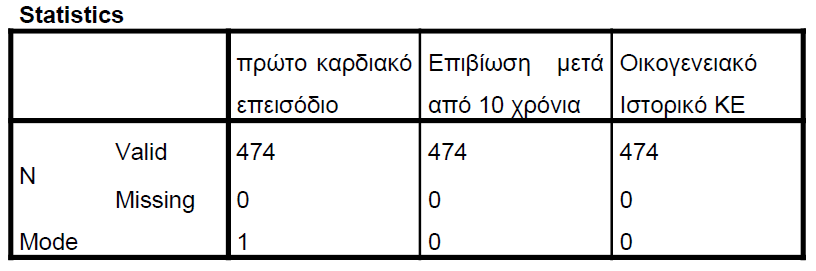
\includegraphics[width=\textwidth]{images/1.PNG}
                      \end{subfigure}
                      
     \begin{subfigure}{0.8\textwidth}
     \centering
         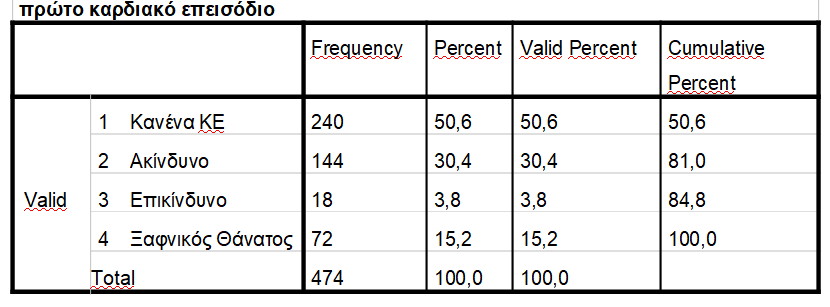
\includegraphics[width=\textwidth]{images/2.PNG}
                      \end{subfigure}
    \end{figure}
    
    \clearpage
    \begin{figure}[ht]
     \centering
     \begin{subfigure}[ht]{0.8\textwidth}
     \centering
         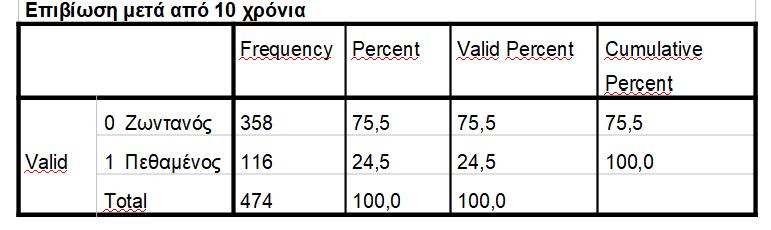
\includegraphics[width=\textwidth]{images/3.PNG}
              \end{subfigure}
     
     \begin{subfigure}[ht]{0.8\textwidth}
     \centering
         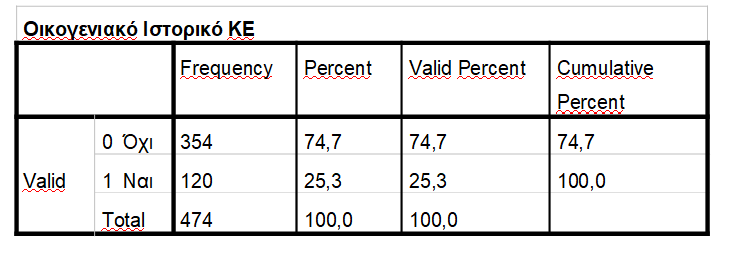
\includegraphics[width=\textwidth]{images/4.PNG}
             \end{subfigure}
      
\end{figure}

Από τους παραπάνω πίνακες παρατηρούμε τα εξής:
\begin{itemize}
    \item Για το πρώτο καρδιακό επεισόδιο η μεταβλητή με τη μεγαλύτερη συχνότητα εμφάνισης είναι η κατηγορία με τον κωδικό 1 = Κανένα ΚΕ και ποσοστό 50,6 \%.
    \item Για την Επιβίωση μετά από 10 χρόνια η μεταβλητή με τη μεγαλύτερη συχνότητα εμφάνισης είναι η κατηγορία με τον κωδικό 0 = Ζωντανός και ποσοστό 75,5 \%.
    \item Για το Οικογενειακό ιστορικό ΚΕ η μεταβλητή με τη μεγαλύτερη συχνότητα εμφάνισης είναι η κατηγορία με τον κωδικό 0 = Όχι και ποσοστό 74,7 \%.
    
\end{itemize}


Τα παραπάνω συμπεράσματα για τις κατηγορικές μεταβλητές επαληθεύονται και από τα ακόλουθα ραβδογράμματα και \lat{Pie charts}.

\clearpage

\begin{figure}[hb]
 \centering
            \begin{subfigure}{0.7\textwidth}
     \centering
         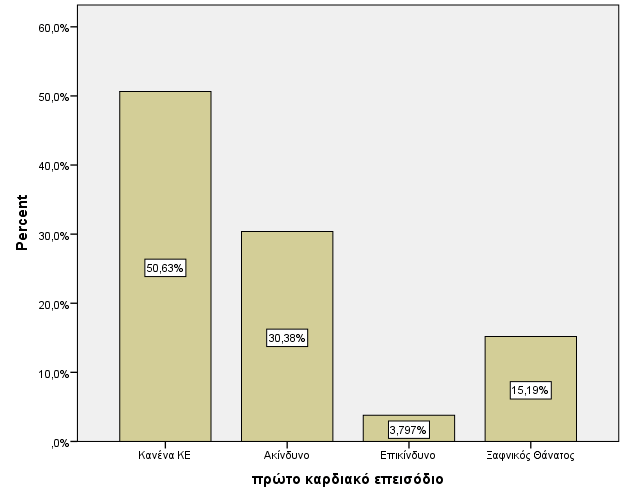
\includegraphics[width=\textwidth]{images/5.png}
                      \end{subfigure}
                       
     \begin{subfigure}{0.6\textwidth}
     \centering
     \vspace{2cm}
         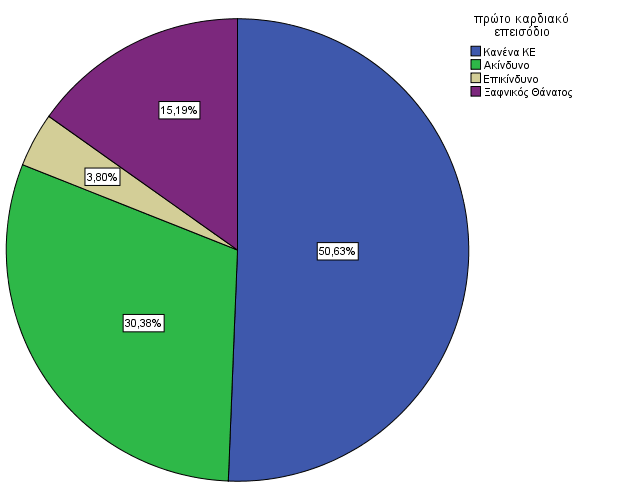
\includegraphics[width=\textwidth]{images/6.png}
                      \end{subfigure}
    \end{figure}

\clearpage
\begin{figure}
 \centering
            \begin{subfigure}{0.7\textwidth}
     \centering
         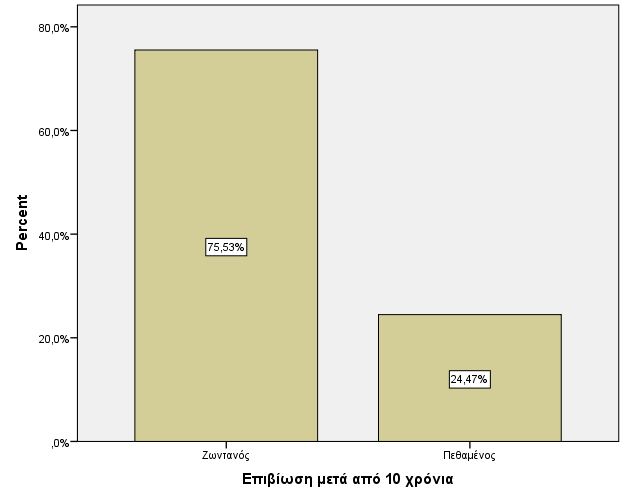
\includegraphics[width=\textwidth]{images/7.png}
                      \end{subfigure}
                      
     \begin{subfigure}{0.6\textwidth}
     \centering
     \vspace{2cm}
         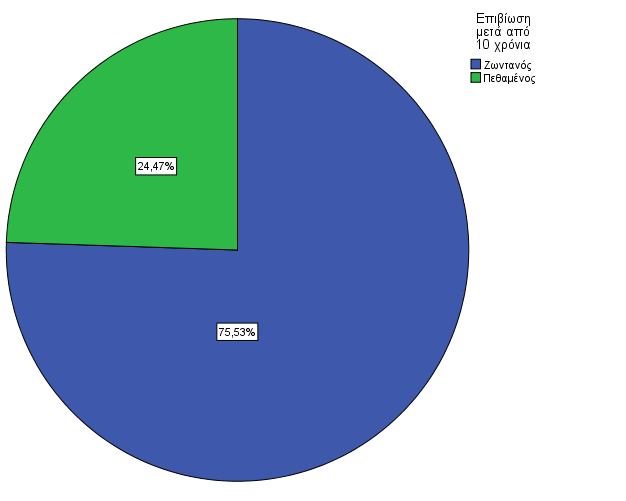
\includegraphics[width=\textwidth]{images/8.png}
                      \end{subfigure}
    \end{figure}
    
    \clearpage
\begin{figure}
 \centering
            \begin{subfigure}{0.7\textwidth}
     \centering
         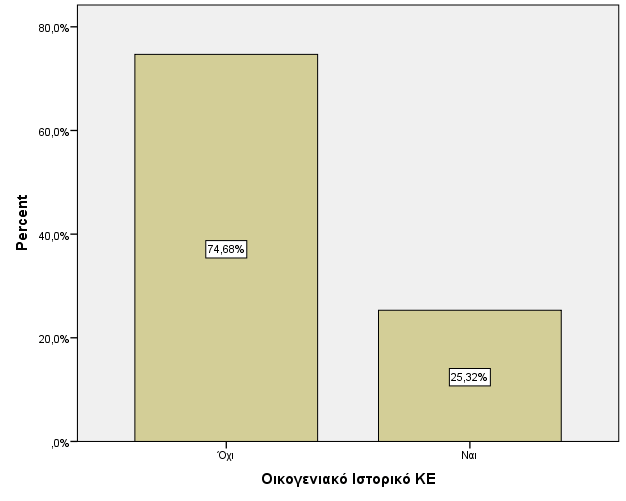
\includegraphics[width=\textwidth]{images/9.png}
                      \end{subfigure}
                      
     \begin{subfigure}{0.6\textwidth}
     \centering
     \vspace{2cm}
         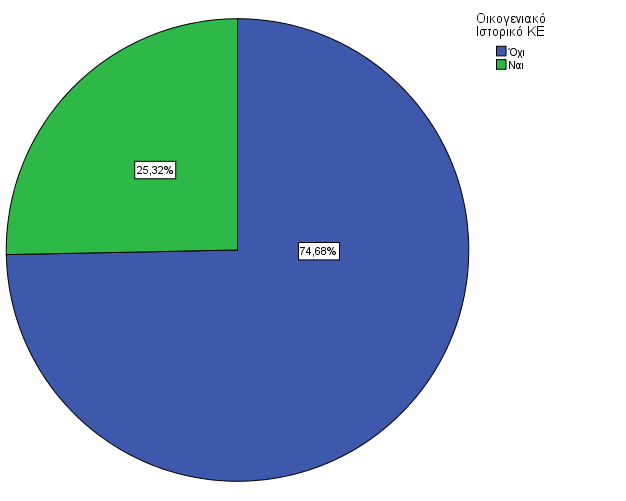
\includegraphics[width=\textwidth]{images/10.png}
                      \end{subfigure}
    \end{figure}
   
   \clearpage 
    Στον ακόλουθο πίνακα παρουσιάζονται όλα τα μέτρα θέσης , διασποράς και μορφής για τις scale μεταβλητές της στατιστικής μας ανάλυσης.
    
    \begin{figure}[hb]
        \centering
        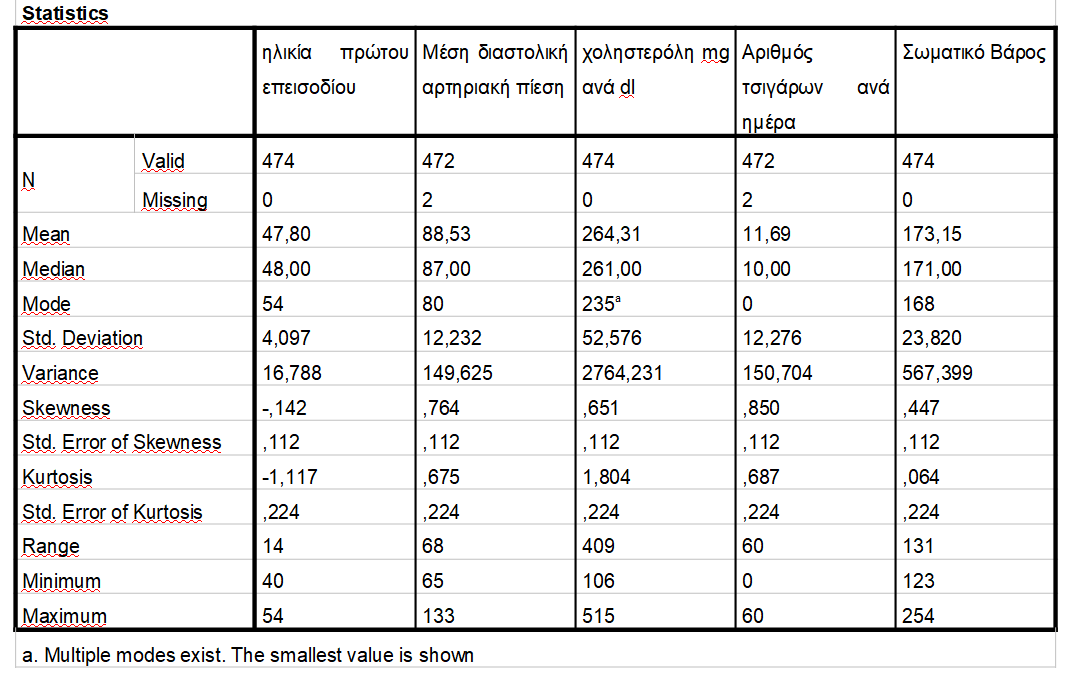
\includegraphics[width=\textwidth]{images/11.PNG}
    \end{figure}
    
    Για τη μεταβλητή ηλικία πρώτου επεισοδίου παρατηρούμε πως ο συντελεστής  skewness είναι αρνητικός (-0,142) , για τη μέση διαστολική αρτηριακή πίεση είναι θετικός (+0,764) όπως και για τη χοληστερόλη (+0,651) , τον αριθμό τσιγάρων ανά ημέρα (+0,850) και το σωματικό βάρος (+0,447) . Όταν ο συγκεκριμένος συντελεστής έχει αρνητική τιμή η κορυφή της κατανομής μετατοπίζεται προς τα δεξιά ενώ όταν έχει θετική τιμή μετατοπίζεται προς τα αριστερά. Επιπλέον η συσσώρευση των παρατηρήσεων προς τα αριστερά ή δεξιά της κατανομής εξετάζεται και μέσω της σύγκρισης των μέτρων της μέσης (mean) και της ενδιάμεσης τιμής (median). Εάν η μέση τιμή είναι μικρότερη της ενδιάμεσης τότε έχουμε αρνητική συμμετρία, ενώ εάν είναι μεγαλύτερη έχουμε θετική συμμετρία, πράγμα το οποίο αποδεικνύεται και από τον πίνακα.

Για τη μεταβλητή ηλικία πρώτου επεισοδίου παρατηρούμε πως ο συντελεστής  kurtosis είναι αρνητικός (-1,117) , για τη μέση διαστολική αρτηριακή πίεση είναι θετικός (+0,675) όπως και για τη χοληστερόλη (+1,804) , τον αριθμό τσιγάρων ανά ημέρα (+0,687) και το σωματικό βάρος (+0,064) . Όταν ο συγκεκριμένος συντελεστής έχει αρνητική τιμή η κατανομή μπορεί να θεωρηθεί πλατύκυρτη, ενώ όταν έχει θετική τιμή μπορεί να θεωρηθεί λεπτόκυρτη.

Σημειώνεται πως οι τιμές των συντελεστών ασυμμετρίας και κύρτωσης πρέπει να βρίσκονται μέσα στο διάστημα -2 έως 2, κάτι το οποίο τηρείται και από τα δεδομένα του πίνακα.


Τα παραπάνω συμπεράσματα για το συντελεστή skewness και kurtosis για τις ποσοτικές μεταβλητές επαληθεύονται και από τα ακόλουθα ιστογράμματα.

\begin{figure}[hb]
 \centering
            \begin{subfigure}{0.65\textwidth}
     \centering
         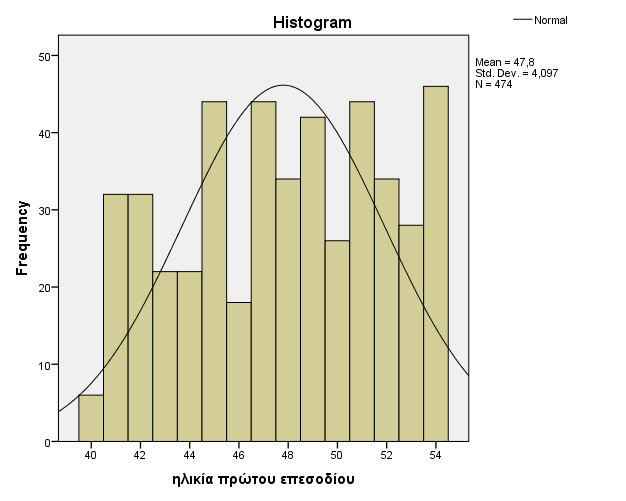
\includegraphics[width=\textwidth]{images/12.png}
                      \end{subfigure}
                     
     \begin{subfigure}{0.65\textwidth}
     \centering
     \vspace{0.5cm}
         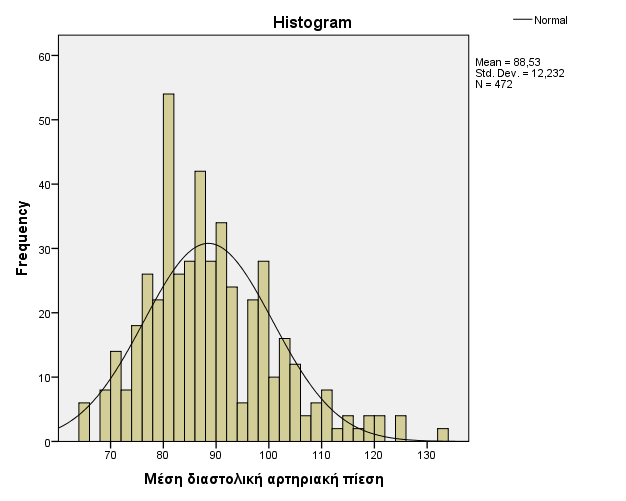
\includegraphics[width=\textwidth]{images/13.png}
                      \end{subfigure}
    \end{figure}
    
    \clearpage
    \begin{figure}
 \centering
            \begin{subfigure}{0.7\textwidth}
     \centering
         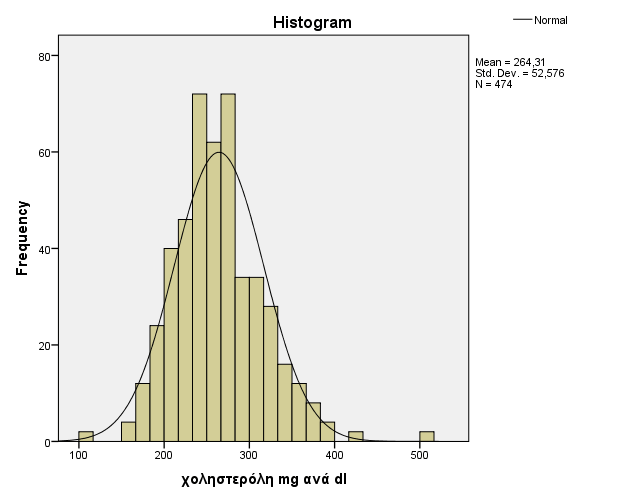
\includegraphics[width=\textwidth]{images/14.png}
                      \end{subfigure}
                      
     \begin{subfigure}{0.7\textwidth}
     \centering
     \vspace{0.5cm}
         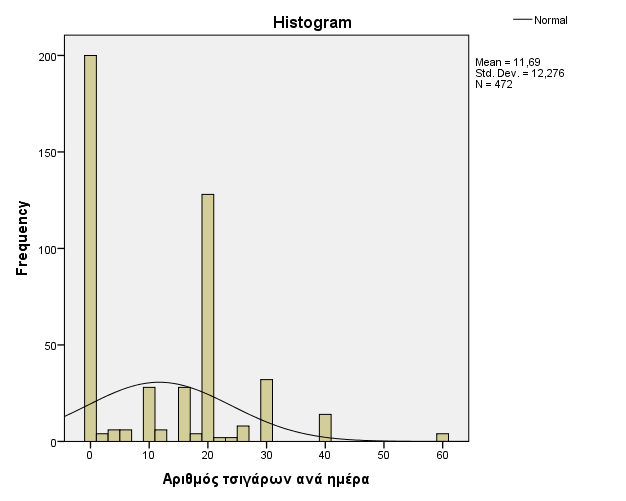
\includegraphics[width=\textwidth]{images/15.png}
                      \end{subfigure}
    \end{figure}
    
    \clearpage
    
    \vspace{0.5cm}
    
    \begin{figure}
        \centering
        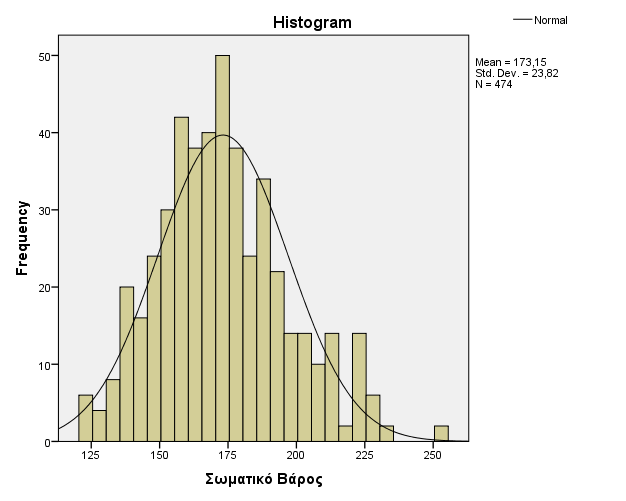
\includegraphics[width=0.7\textwidth]{images/16.png}
    \end{figure}
    
    Στη συνέχεια παρατίθενται τα θηκογράμματα των ποσοτικών μεταβλητών. Όπως παρατηρείται δεν υπάρχουν εξαιρετικά ακραίες τιμές (outliers – δηλαδή τιμές που ξεπερνάνε κατά 1,5 ή κατά 3 φορές το ενδοτεταρτημοριακό εύρος) μόνο για τη μεταβλητή  “Ηλικία πρώτου επεισοδίου”. 
    
    \clearpage
    \begin{figure}
 \centering
            \begin{subfigure}{0.7\textwidth}
     \centering
         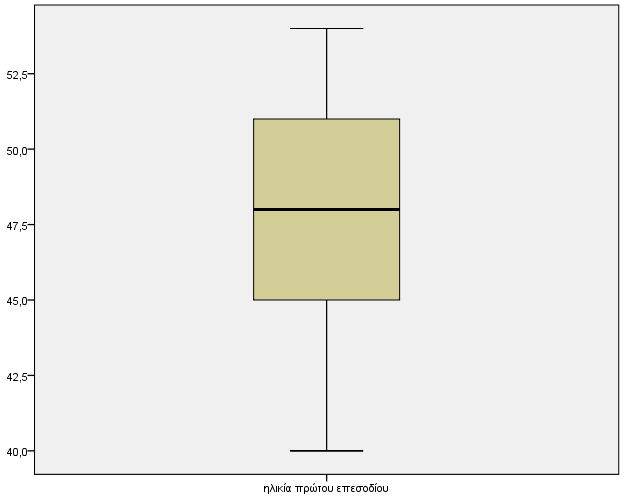
\includegraphics[width=\textwidth]{images/17.png}
                      \end{subfigure}
                      
     \begin{subfigure}{0.7\textwidth}
     \centering
      \vspace{1cm}
         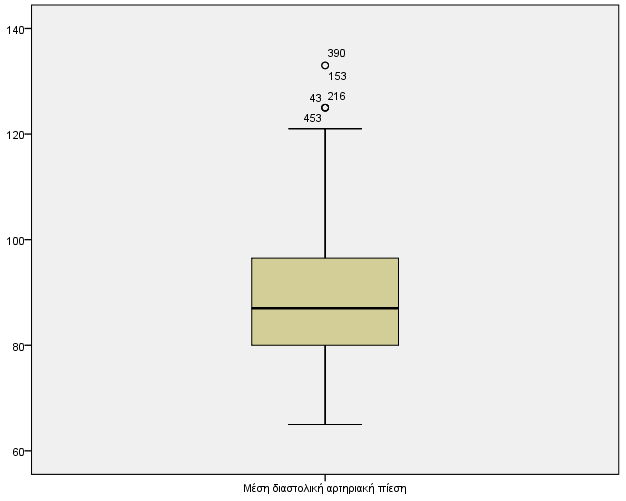
\includegraphics[width=\textwidth]{images/18.png}
                      \end{subfigure}
    \end{figure}
    
   \clearpage
    \begin{figure}
 \centering
            \begin{subfigure}{0.7\textwidth}
     \centering
         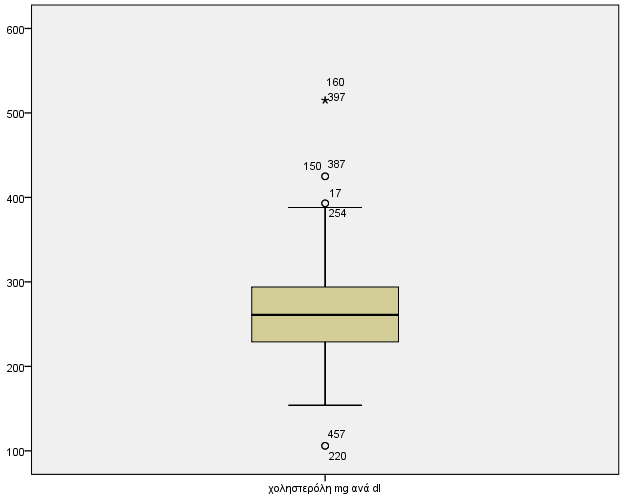
\includegraphics[width=\textwidth]{images/19.png}
                      \end{subfigure}
                      
     \begin{subfigure}{0.7\textwidth}
     \centering
     \vspace{1cm}
         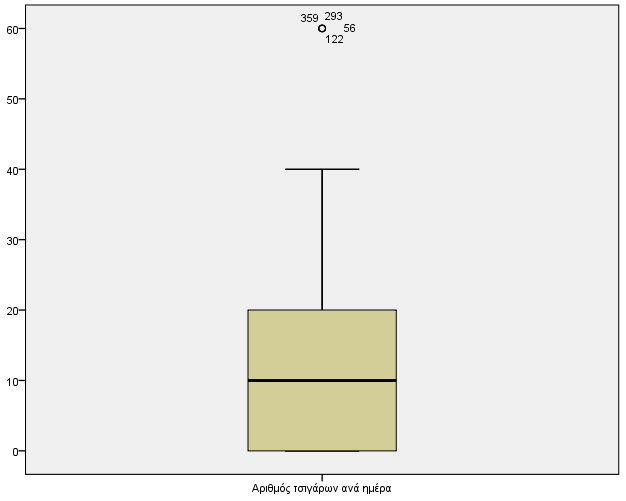
\includegraphics[width=\textwidth]{images/20.png}
                      \end{subfigure}
    \end{figure}
    
    \begin{figure}
        \centering
        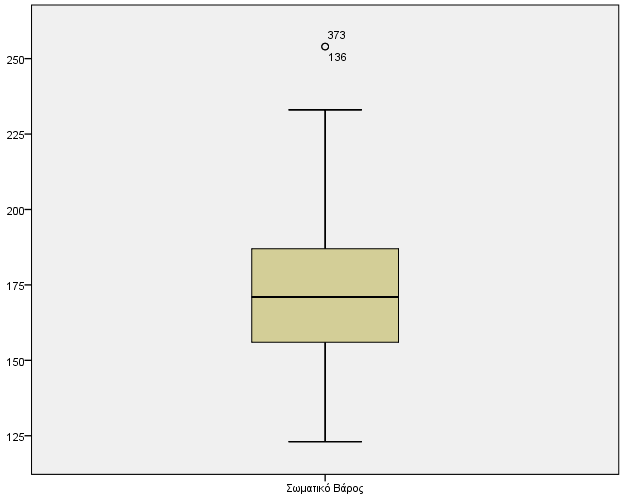
\includegraphics[width=0.7\textwidth]{images/21.png}
    \end{figure}
    
\clearpage
Στον ακόλουθο πίνακα παρουσιάζονται τα προεπιλεγμένα περιγραφικά στατιστικά στοιχεία για τη “Μέση διαστολική αρτηριακή πίεση” ανά κατηγορίες σοβαρότητας πρώτου καρδιακού επεισοδίου και οικογενειακού ιστορικού ΚΕ.
\begin{figure}[hb]
        \centering
        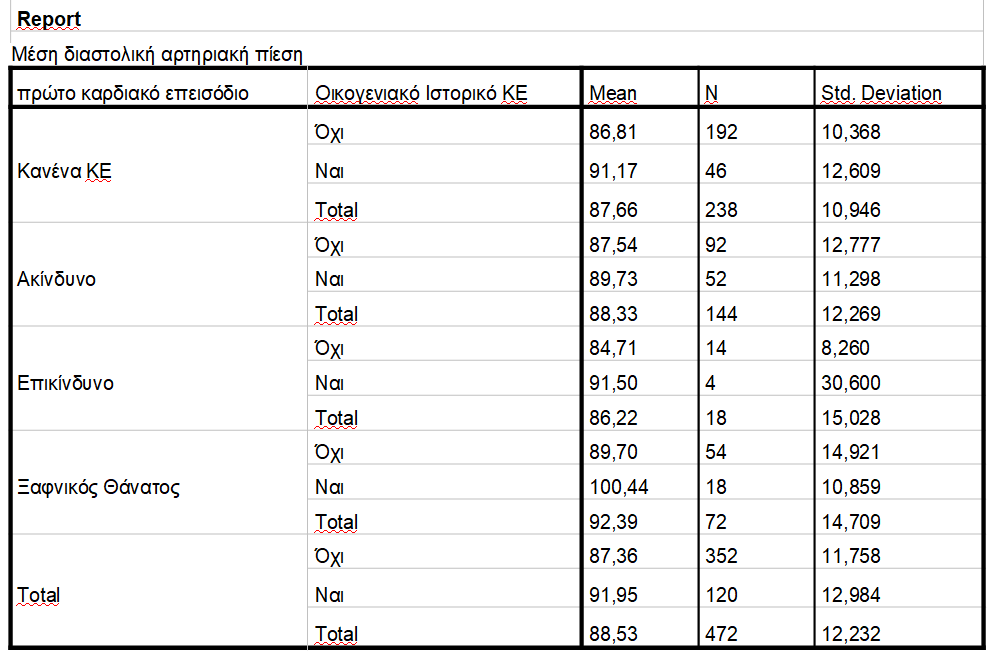
\includegraphics[width=0.7\textwidth]{images/22.PNG}
    \end{figure}
    
    Από τα στοιχεία του πίνακα παρατηρούμε πως τα άτομα τα οποία δεν έχουν οικογενειακό ιστορικό παρουσιάζουνε μικρότερες τιμές μέσης διαστολικής αρτηριακής πίεσης για όλες τις κατηγορίες της μεταβλητής “ πρώτο καρδιακό επεισόδιο “ . 
    
Επιπλέον φαίνεται να μην υπάρχει κάποια συστηματική αύξηση της μέσης διαστολικής αρτηριακής πίεσης για τις κατηγορίες του πρώτου καρδιακού επεισοδίου στο υπό μελέτη δείγμα. Το μόνο που μπορούμε να παρατηρήσουμε είναι πως τα άτομα της κατηγορίας ξαφνικός θάνατος έχουν την μεγαλύτερη τιμή μέσης διαστολικής αρτηριακής πίεσης (Total = 92,39). 

Τέλος,  παρατηρώντας τη στήλη που παρουσιάζει την τυπική απόκλιση της μέσης διαστολικής αρτηριακής πίεσης αξίζει να αναφερθεί ότι η μεγαλύτερη διασπορά γύρω από τη μέση διαστολική αρτηριακή πίεση εμφανίζεται στα άτομα με οικογενειακό ιστορικό στην κατηγορία επικίνδυνο ΚΕ (st.dev = 30,60).  

\clearpage
Στον ακόλουθο πίνακα παρουσιάζονται τα προεπιλεγμένα περιγραφικά στατιστικά στοιχεία για τη “Μέση διαστολική αρτηριακή πίεση” ανά κατηγορίες σοβαρότητας πρώτου καρδιακού επεισοδίου και επιβίωσης μετά από 10 χρόνια.

\begin{figure}[hb]
        \centering
        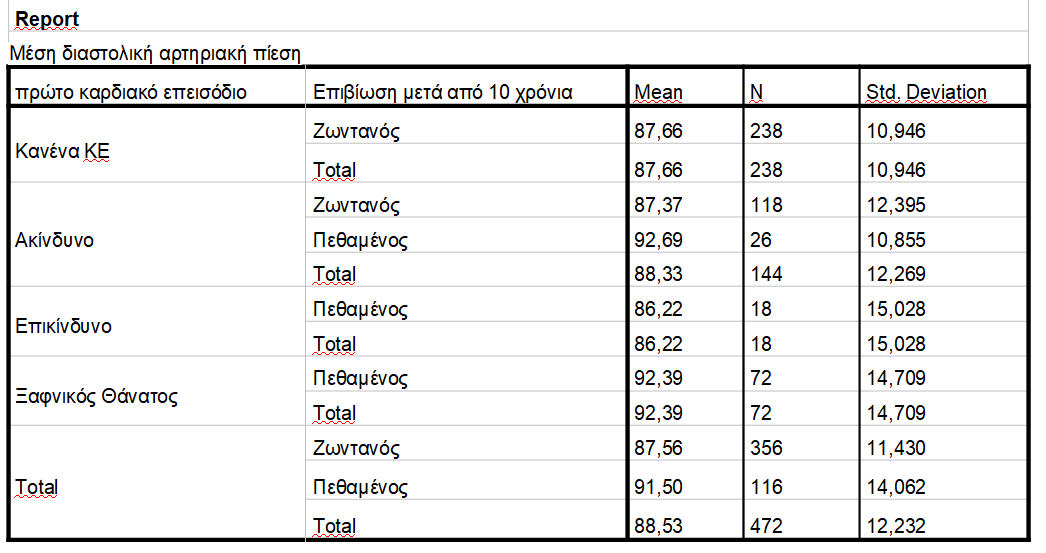
\includegraphics[width=0.7\textwidth]{images/23.PNG}
    \end{figure}
    
    Από τα στοιχεία του πίνακα παρατηρούμε πως στις κατηγορίες επικίνδυνο και ξαφνικός θάνατος της μεταβλητής πρώτο καρδιακό επεισόδιο δεν έχει επιβιώσει κανένας μετά από 10 χρόνια.
    
Επιπλέον φαίνεται να μην υπάρχει κάποια συστηματική αύξηση της μέσης διαστολικής αρτηριακής πίεσης για τις κατηγορίες του πρώτου καρδιακού επεισοδίου στο υπό μελέτη δείγμα. Το μόνο που μπορούμε να παρατηρήσουμε είναι πως τα άτομα της κατηγορίας ξαφνικός θάνατος έχουν την μεγαλύτερη τιμή μέσης διαστολικής αρτηριακής πίεσης (Total$=$92,39).  Στην επόμενη παράγραφο θα εξεταστεί αν οι διαφορές είναι στατιστικά σημαντικές.

Τέλος,  παρατηρώντας τη στήλη που παρουσιάζει την τυπική απόκλιση της μέσης διαστολικής αρτηριακής πίεσης αξίζει να αναφερθεί ότι η μεγαλύτερη διασπορά  εμφανίζεται στα άτομα τα οποία δεν έχουν επιβιώσει μετά από 10 χρόνια στην κατηγορία επικίνδυνο ΚΕ (st.dev = 15,028). 

\clearpage
Στον ακόλουθο πίνακα παρουσιάζονται τα προεπιλεγμένα περιγραφικά στατιστικά στοιχεία για τη “χοληστερόλη” ανά κατηγορίες σοβαρότητας πρώτου καρδιακού επεισοδίου και Οικογενειακό ιστορικό ΚΕ.

\begin{figure}[hb]
        \centering
        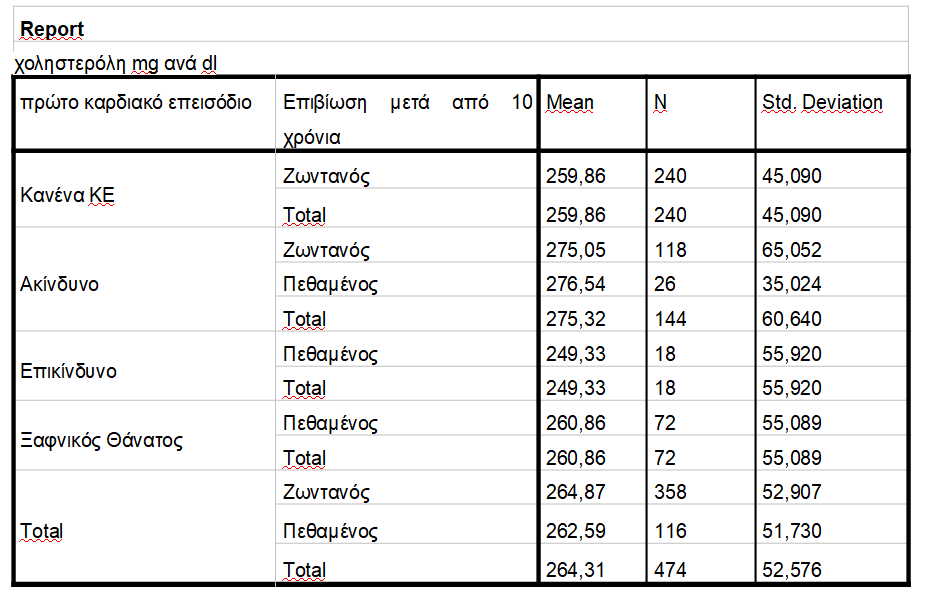
\includegraphics[width=0.7\textwidth]{images/24.PNG}
    \end{figure}
    
Από τα στοιχεία του πίνακα παρατηρούμε πως η μεγαλύτερη μέση τιμή για τη μεταβλητή χοληστερόλη παρατηρείται στα άτομα τα οποία δεν έχουν επιβιώσει μετά από 10 χρόνια για την κατηγορία ακίνδυνο της μεταβλητής πρώτο καρδιακό επεισόδιο (276,54) . 
Τέλος,  παρατηρώντας τη στήλη που παρουσιάζει την τυπική απόκλιση της χοληστερόλης αξίζει να αναφερθεί ότι η μεγαλύτερη διασπορά εμφανίζεται στα άτομα τα οποία έχουν επιβιώσει μετά από 10 χρόνια στην κατηγορία ακίνδυνο ΚΕ (st.dev = 65,052).

\clearpage
Στον ακόλουθο πίνακα παρουσιάζονται τα προεπιλεγμένα περιγραφικά στατιστικά στοιχεία για τη “Σωματικό Βάρος” ανά κατηγορίες σοβαρότητας πρώτου καρδιακού επεισοδίου και επιβίωσης μετά από 10 χρόνια.
\begin{figure}[hb]
        \centering
        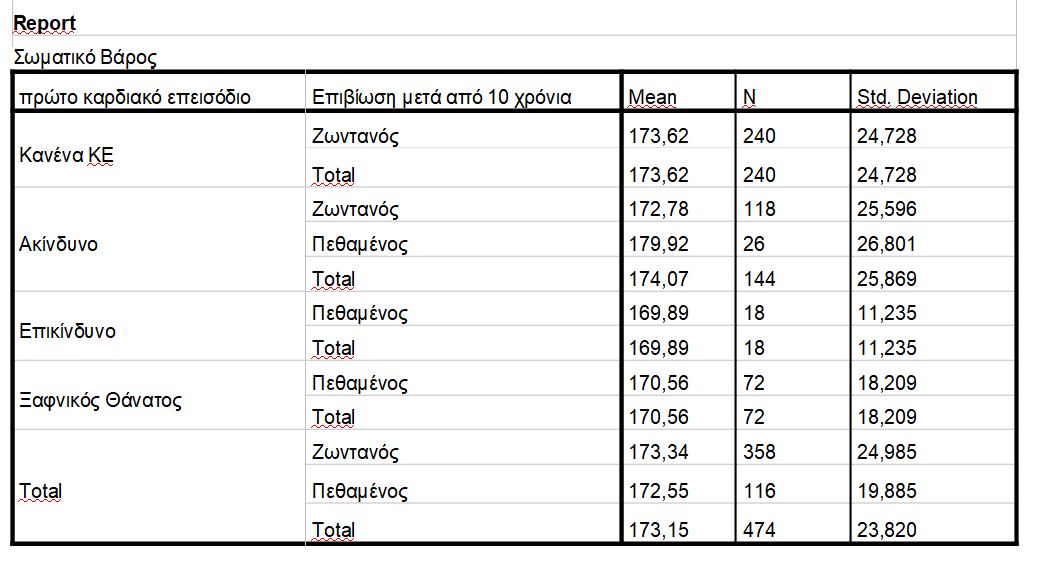
\includegraphics[width=0.7\textwidth]{images/25.PNG}
    \end{figure}
    
    Από τον πίνακα παρατηρούμε πως η μεγαλύτερη μέση τιμή για το Σωματικό Βάρος αναφέρεται στα άτομα τα οποία δεν έχουν επιβιώσει μετά από 10 χρόνια στην κατηγορία ακίνδυνο της μεταβλητής πρώτο καρδιακό επεισόδιο.
    
Επιπλέον φαίνεται να μην υπάρχει κάποια συστηματική αύξηση του Σωματικού Βάρους  για τις κατηγορίες του πρώτου καρδιακού επεισοδίου στο υπό μελέτη δείγμα. Το μόνο που μπορούμε να παρατηρήσουμε είναι πως τα άτομα της κατηγορίας ακίνδυνο έχουν την μεγαλύτερη τιμή Σωματικού Βάρους (Total = 174,07). 

Τέλος,  παρατηρώντας τη στήλη που παρουσιάζει την τυπική απόκλιση του Σωματικού Βάρους αξίζει να αναφερθεί ότι η μεγαλύτερη διασπορά εμφανίζεται στα άτομα τα οποία δεν έχουν επιβιώσει μετά από 10 χρόνια στην κατηγορία ακίνδυνο ΚΕ (st.dev = 26,801).

\clearpage
Στον ακόλουθο πίνακα παρουσιάζονται τα προεπιλεγμένα περιγραφικά στατιστικά στοιχεία για τον “Αριθμό τσιγάρων” ανά κατηγορίες σοβαρότητας πρώτου καρδιακού επεισοδίου και επιβίωσης μετά από 10 χρόνια.

\begin{figure}[hb]
        \centering
        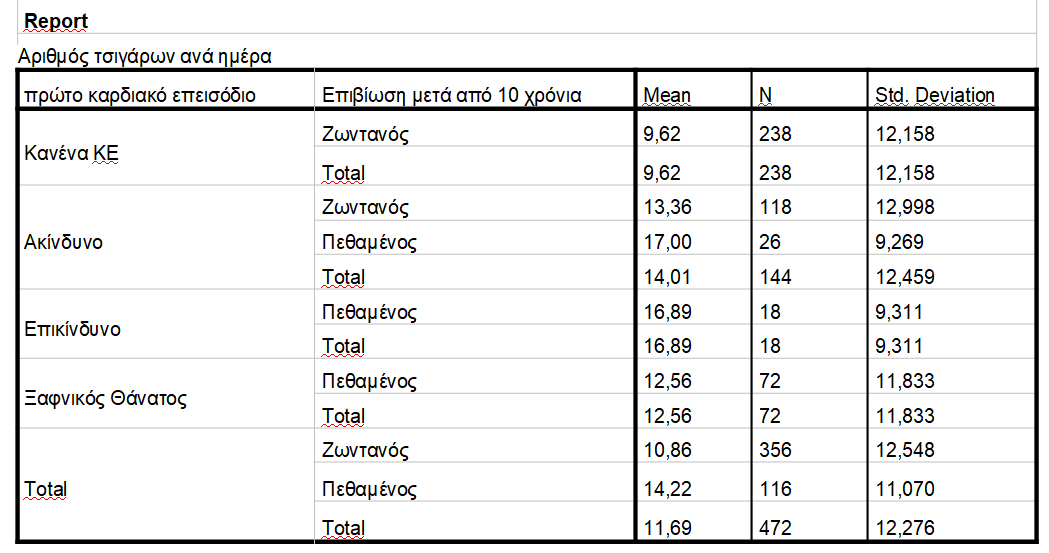
\includegraphics[width=0.7\textwidth]{images/26.PNG}
    \end{figure}
    
Από τον πίνακα φαίνεται να μην υπάρχει κάποια συστηματική αύξηση του Αριθμού τσιγάρων ανά ημέρα  για τις κατηγορίες του πρώτου καρδιακού επεισοδίου στο υπό μελέτη δείγμα. Παρ’ όλα αυτά φαίνεται να υπάρχουν στατιστικά σημαντικές διαφορές στις μέσες τιμές, κάτι το οποίο θα εξεταστεί στη συνέχεια της εργασίας. Το μόνο που μπορούμε να παρατηρήσουμε είναι πως τα άτομα της κατηγορίας επικίνδυνο πρώτο καρδιακό επεισόδιο έχουν την μεγαλύτερη τιμή Αριθμού τσιγάρων ανά ημέρα (Total = 16,89). 

Όσον αφορά τη σχέση της επιβίωσης μετά από 10 χρόνια με τον αριθμό των τσιγάρων ανά ημέρα, φαίνεται ότι όσοι δεν επιβίωσαν κάπνιζαν περισσότερο σε σχέση με αυτούς που επέζησαν. Η διαφορά αυτή στις μέσες τιμές θα εξεταστεί και παρακάτω. 

\clearpage
Ακολούθως, παρατίθενται τα συνδυαστικά διαγράμματα (clustered) μεταξύ των κατηγορικών μεταβλητών πρώτο καρδιακό επεισόδιο – επιβίωση μετά από 10 χρόνια – οικογενειακό ιστορικό ΚΕ.  
\begin{figure}[hb]
        \centering
        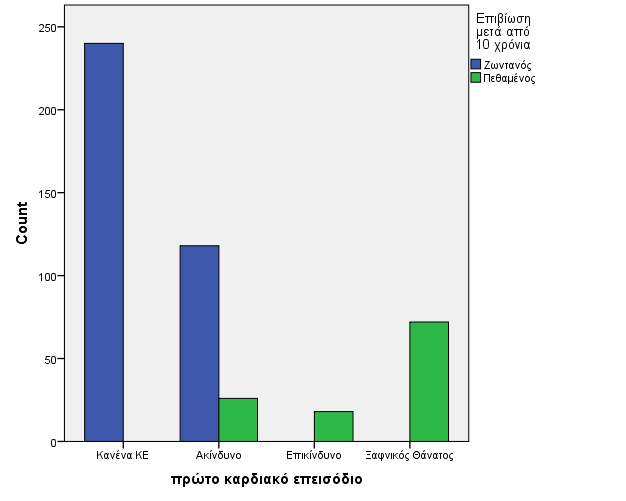
\includegraphics[width=0.8\textwidth]{images/27.png}
    \end{figure}
    
    Από το πρώτο συνδυαστικό διάγραμμα διαπιστώνουμε ότι το ποσοστό των ατόμων που έχουν επιβιώσει μετά από 10 χρόνια είναι πολύ μεγαλύτερο από αυτό των θανόντων για ακίνδυνο πρώτο καρδιακό επεισόδιο, ενώ στην υποκατηγορία επικίνδυνο δεν έχει επιβιώσει κανείς.  
    
    \clearpage
    \begin{figure}[hb]
        \centering
        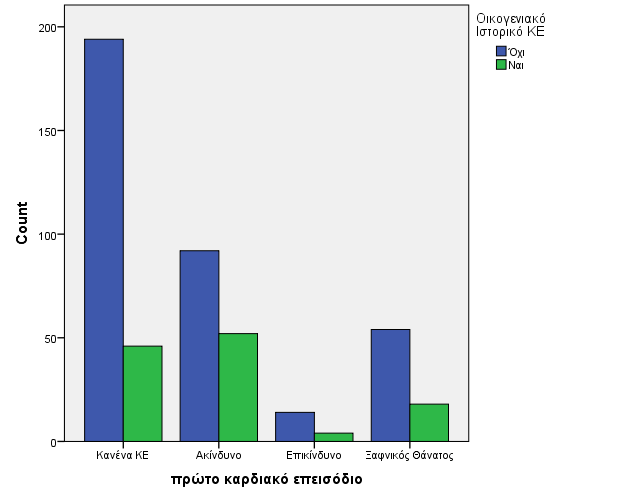
\includegraphics[width=0.8\textwidth]{images/28.png}
    \end{figure}
    Στο δεύτερο συνδυαστικό διάγραμμα αξίζει να τονιστεί ότι τα άτομα τα οποία δεν έχουν οικογενειακό ιστορικό και έχουν υποστεί ακίνδυνο, επικίνδυνο και ξαφνικό θάνατο λόγω πρώτου καρδιακού επεισοδίου είναι περισσότερα σε σχέση με αυτά που έχουν οικογενειακό ιστορικό.
    
    \clearpage
    \begin{figure}[hb]
        \centering
        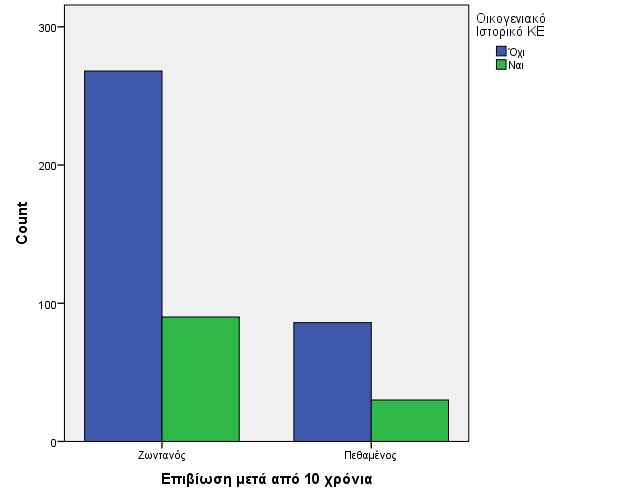
\includegraphics[width=0.8\textwidth]{images/29.png}
    \end{figure}
    
    Στο τρίτο συνδυαστικό διάγραμμα διαπιστώνεται ότι στα άτομα που δεν έχουν επιβιώσει μετά από 10 χρόνια μετά από καρδιακό επεισόδιο τα περισσότερα δεν είχαν οικογενειακό ιστορικό ΚΕ.  